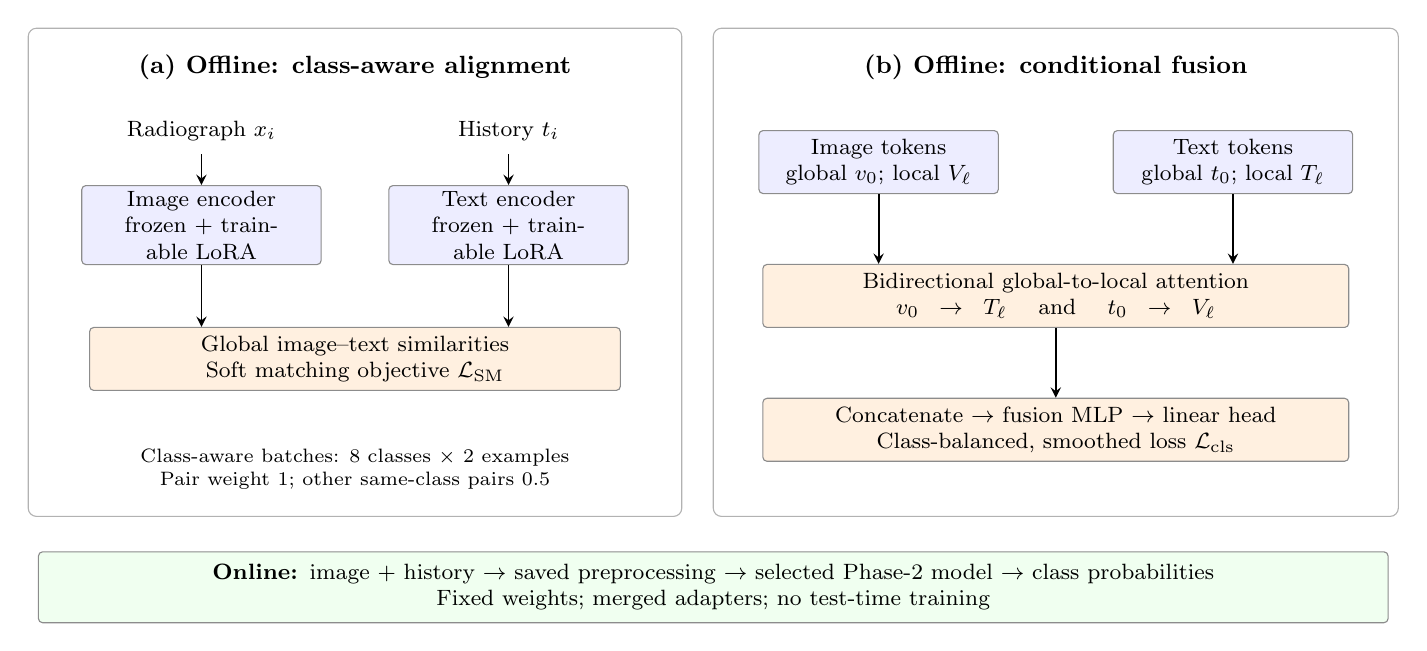
\begin{tikzpicture}[x=1mm,y=1mm,font=\footnotesize,
box/.style={draw=black!45,rounded corners=1.5pt,align=center,minimum height=8mm,inner sep=2pt},
flow/.style={->,>=stealth,line width=.65pt},
enc/.style={box,fill=blue!7,text width=29mm},
learn/.style={box,fill=orange!12},
note/.style={font=\scriptsize,align=center}]
\draw[rounded corners=3pt,draw=black!30] (0,0) rectangle (83,62);
\draw[rounded corners=3pt,draw=black!30] (87,0) rectangle (174,62);
\node[font=\small\bfseries] at (41.5,57) {(a) Offline: class-aware alignment};
\node[font=\small\bfseries] at (130.5,57) {(b) Offline: conditional fusion};
\node at (22,49) {Radiograph $x_i$};
\node at (61,49) {History $t_i$};
\node[enc] (vi) at (22,37) {Image encoder\\frozen + trainable LoRA};
\node[enc] (ti) at (61,37) {Text encoder\\frozen + trainable LoRA};
\draw[flow] (22,46) -- (vi);
\draw[flow] (61,46) -- (ti);
\node[learn,text width=66mm] (align) at (41.5,20) {Global image--text similarities\\Soft matching objective $\mathcal L_{\mathrm{SM}}$};
\draw[flow] (vi.south) -- (align.north -| vi.south);
\draw[flow] (ti.south) -- (align.north -| ti.south);
\node[note] at (41.5,6) {Class-aware batches: 8 classes $\times$ 2 examples\\Pair weight 1; other same-class pairs 0.5};
\node[enc] (vf) at (108,45) {Image tokens\\global $v_0$; local $V_\ell$};
\node[enc] (tf) at (153,45) {Text tokens\\global $t_0$; local $T_\ell$};
\node[learn,text width=73mm] (cross) at (130.5,28) {Bidirectional global-to-local attention\\$v_0\!\to\!T_\ell$ \quad and \quad $t_0\!\to\!V_\ell$};
\draw[flow] (vf.south) -- (cross.north -| vf.south);
\draw[flow] (tf.south) -- (cross.north -| tf.south);
\node[learn,text width=73mm] (head) at (130.5,11) {Concatenate $\to$ fusion MLP $\to$ linear head\\Class-balanced, smoothed loss $\mathcal L_{\mathrm{cls}}$};
\draw[flow] (cross) -- (head);
\node[box,fill=green!6,text width=170mm,minimum height=9mm] at (87,-9) {\textbf{Online:} image + history $\to$ saved preprocessing $\to$ selected Phase-2 model $\to$ class probabilities\\Fixed weights; merged adapters; no test-time training};
\end{tikzpicture}
